\documentclass[a4paper, 11pt, english]{article}
\usepackage[margin=0.8in]{geometry}
\usepackage{amsmath}
\usepackage{amssymb}
\usepackage{amsfonts}
\usepackage{fancyhdr}
\usepackage{listings}
\usepackage[american, siunitx]{circuitikz}
\usepackage{tikz-timing}
\usepackage{float}
\usepackage{graphicx}
\usepackage{amsthm}
\usepackage{color}
\usepackage[backend=biber]{biblatex}
\addbibresource{ref.bib}
% \usepackage{etoolbox}
% \apptocmd{\sloppy}{\hbadness 10000\relax}{}{}
\lstset
{
  language = {},
  basicstyle = \scriptsize,
  numbers = left,
  stepnumber = 1,
  showstringspaces = false,
  frame = single,
  tabsize = 1,
  breaklines = true,
  breakatwhitespace = false,
}
\pagestyle{fancy}
\lhead{Christopher Dizon \& Nate Kibanoff \& Sir Heinrich Tan\\CS 152B B}
\rhead{MA122.1 Project\\Neural Networks}

\newtheorem{theorem}{Theorem}
\newtheorem{corollary}{Corollary}
\newtheorem{lemma}{Lemma}
\renewcommand\qedsymbol{QED}
% \renewcommand\qedsymbol{$\blacksquare$}
%from external sources
%--------------------------------------------------------------------------------------
%https://tex.stackexchange.com/questions/235118/making-a-thicker-cdot-for-dot-product-that-is-thinner-than-bullet/235120 (Manuel)
\makeatletter
\newcommand*\bigcdot{\mathpalette\bigcdot@{.5}}
\newcommand*\bigcdot@[2]{\mathbin{\vcenter{\hbox{\scalebox{#2}{$\m@th#1\bullet$}}}}}
\makeatother
%--------------------------------------------------------------------------------------

\begin{document}
\section{Introduction}
% intro to neural networks
% provide pictures
% example to put in picture
% \begin{figure}[H]
%   \centering
%   \includegraphics[width=12cm]{filename (in the same folder dapat)}
%   \caption{caption here}
%   \label{fig:label of the figure}
% \end{figure}
Neural networks have a lot of applications in today's world. They have applications in character recognition, image compression, stock market prediction, medicine, and much more \cite{dk1}. They provide us with a way to compute for more complicated things. % pls edit with more pictures

\begin{figure}[H]
  \centering
  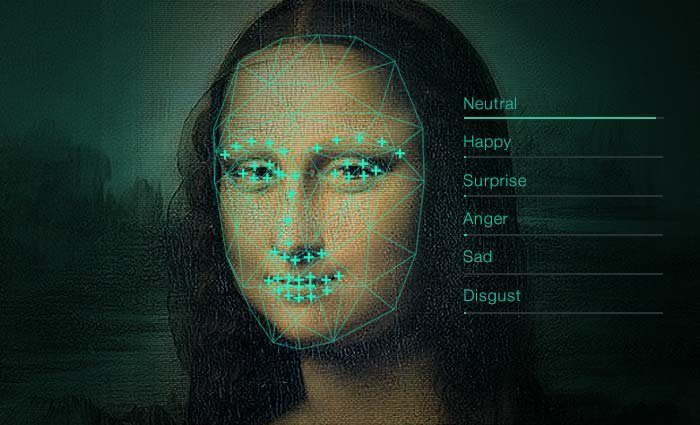
\includegraphics[width=12cm]{images/intro1.jpg}
  \caption{Face Recognition Example \cite{targett_nunns_ball_2018}} % need source
  \label{fig:intro1}
\end{figure}

\par When neural networks are mentioned, people tend to panic as they think it is a very complicated topic. However, it is not incredibly complicated. For people with a background in linear algebra, neural networks become something more tangible, because it is just applying concepts in linear algebra.
\par For this topic, we will discuss a basic kind of neural network. It is not too complicated (like the modern versions of neural networks) and it is easy to follow.

\section{Preliminaries}
% activation functions/sigmoid
\subsection{Activation Function}
\par The activation function is simply a function that squeezes numbers to fit into a certain range. In this case, we try to fit numbers in the range $[0,1]$. There are many kinds of activation functions, and the function we use for this topic is the sigmoid function. The sigmoid function is defined as
\[\sigma(x) = \frac{1}{1+e^{-x}}.\]

% gradient descent
\subsection{Gradient Descent}
\par Gradient descent is an algorithm that "tweaks it's parameters iteratively to minimize a given function to its local minimum \cite{donges_2018}." In essence, it is a way to minimize some type of cost function.
\par Suppose we have a 2-dimensional curve on the Cartesian plane. If we consider any point on the plane, it is possible to determine if there is a downward slope either to the left or to the right of the point by getting the derivative of the function on that point.

\begin{figure}[H]
  \centering
  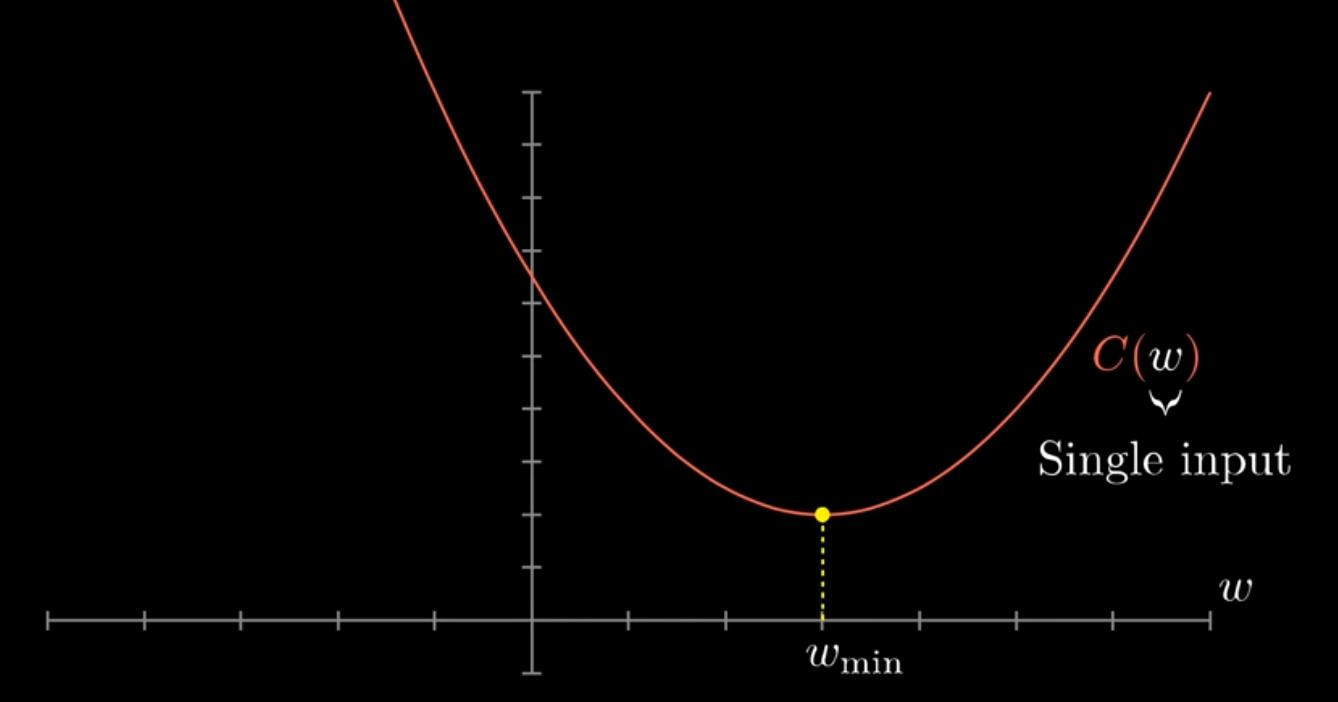
\includegraphics[width=12cm]{images/gd1.jpg}
  \caption{Point at a local minima\cite{3blue1brown_2017_2}}
  \label{fig:gd1}
\end{figure}

\par This is useful because it can also tell us where the point should adjust to in order to get closer to the (or one of the) local minima of the function. Namely, make the point adjust to its left if the slope at that point is positive, and to its right if the slope is negative.

\begin{figure}[H]
  \centering
  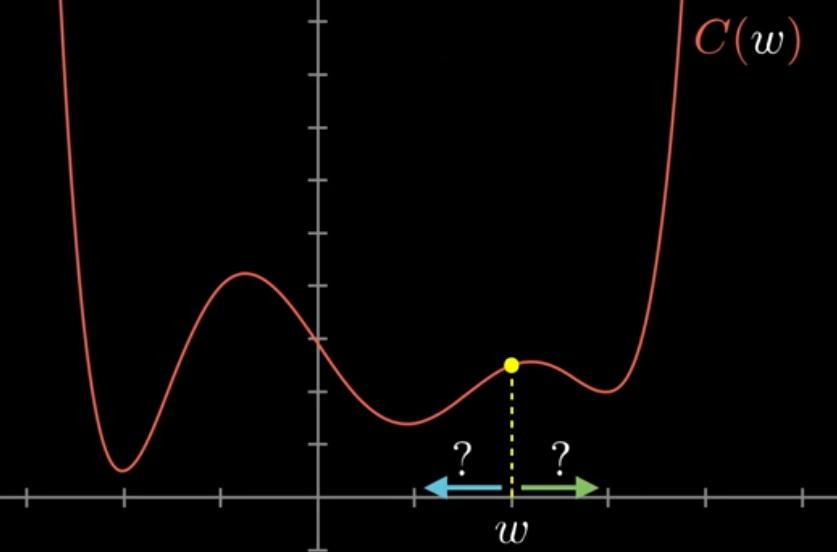
\includegraphics[width=12cm]{images/gd2.jpg}
  \caption{Deciding where to adjust given a point on a curve\cite{3blue1brown_2017_2}}
  \label{fig:gd2}
\end{figure}

\par By extension, this can work for an n-dimensional figure. For example, this could work with a 3-dimensional curve because we could get the partial derivative of each point in the space.

\begin{figure}[H]
  \centering
  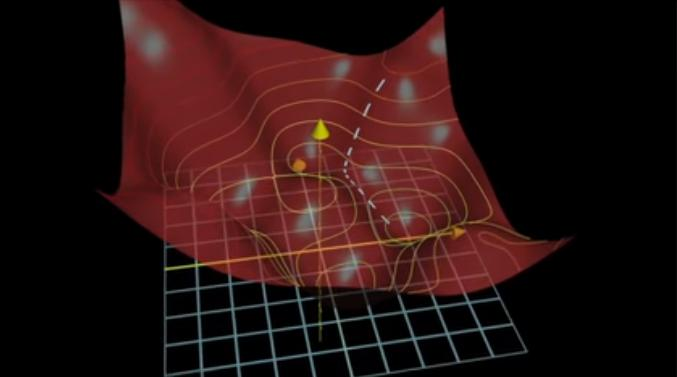
\includegraphics[width=12cm]{images/gd3.jpg}
  \caption{Example of a 3D curve with local minima\cite{3blue1brown_2017_2}}
  \label{fig:gd3}
\end{figure}

\par Thus, for each point, we iteratively adjust it closer to a local minima. When this is applied repeatedly in units proportional to the slope of the curve at each point, you get what is called gradient. This gradient, when configured to move towards a local minima, is called a gradient descent.

\begin{figure}[H]
  \centering
  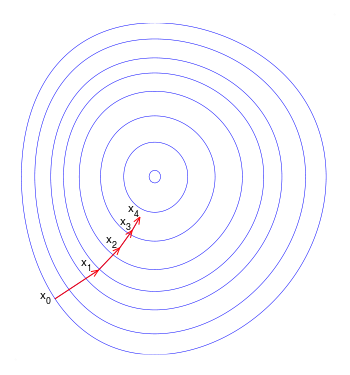
\includegraphics[width=12cm]{images/gd4.png}
  \caption{Iteratively approaching a minimum\cite{3blue1brown_2017_2}}
  \label{fig:gd4}
\end{figure}

% WARNING: NOT DONE; include bias?

\subsection{Definition of Terms}
\par Before discussing how the neural network works, we must define the following terms:
\begin{description}
    \item[Neurons] \hfill \\ These are represented as the nodes in the neural network.
    \item[Layers] \hfill \\ These are the vertical arrangements of neurons in the neural network.
    \item[Weights] \hfill \\ These are represented as the edges  connecting one neuron to the all neurons in the next layer.
\end{description}

\section{Discussion}
% how is linear alg used
\par The neural network is composed of different phases, each having an effect to the actual network. % WARNING: NOT DONE

% forward phase
\subsection{Forward Phase}
\par A neural network consists of an input layer, an arbitrary amount of hidden layers, and an output layer. Each layer consists of an arbitrary amount of neurons depending on the purpose of the neural network.

\begin{figure}[H]
  \centering
  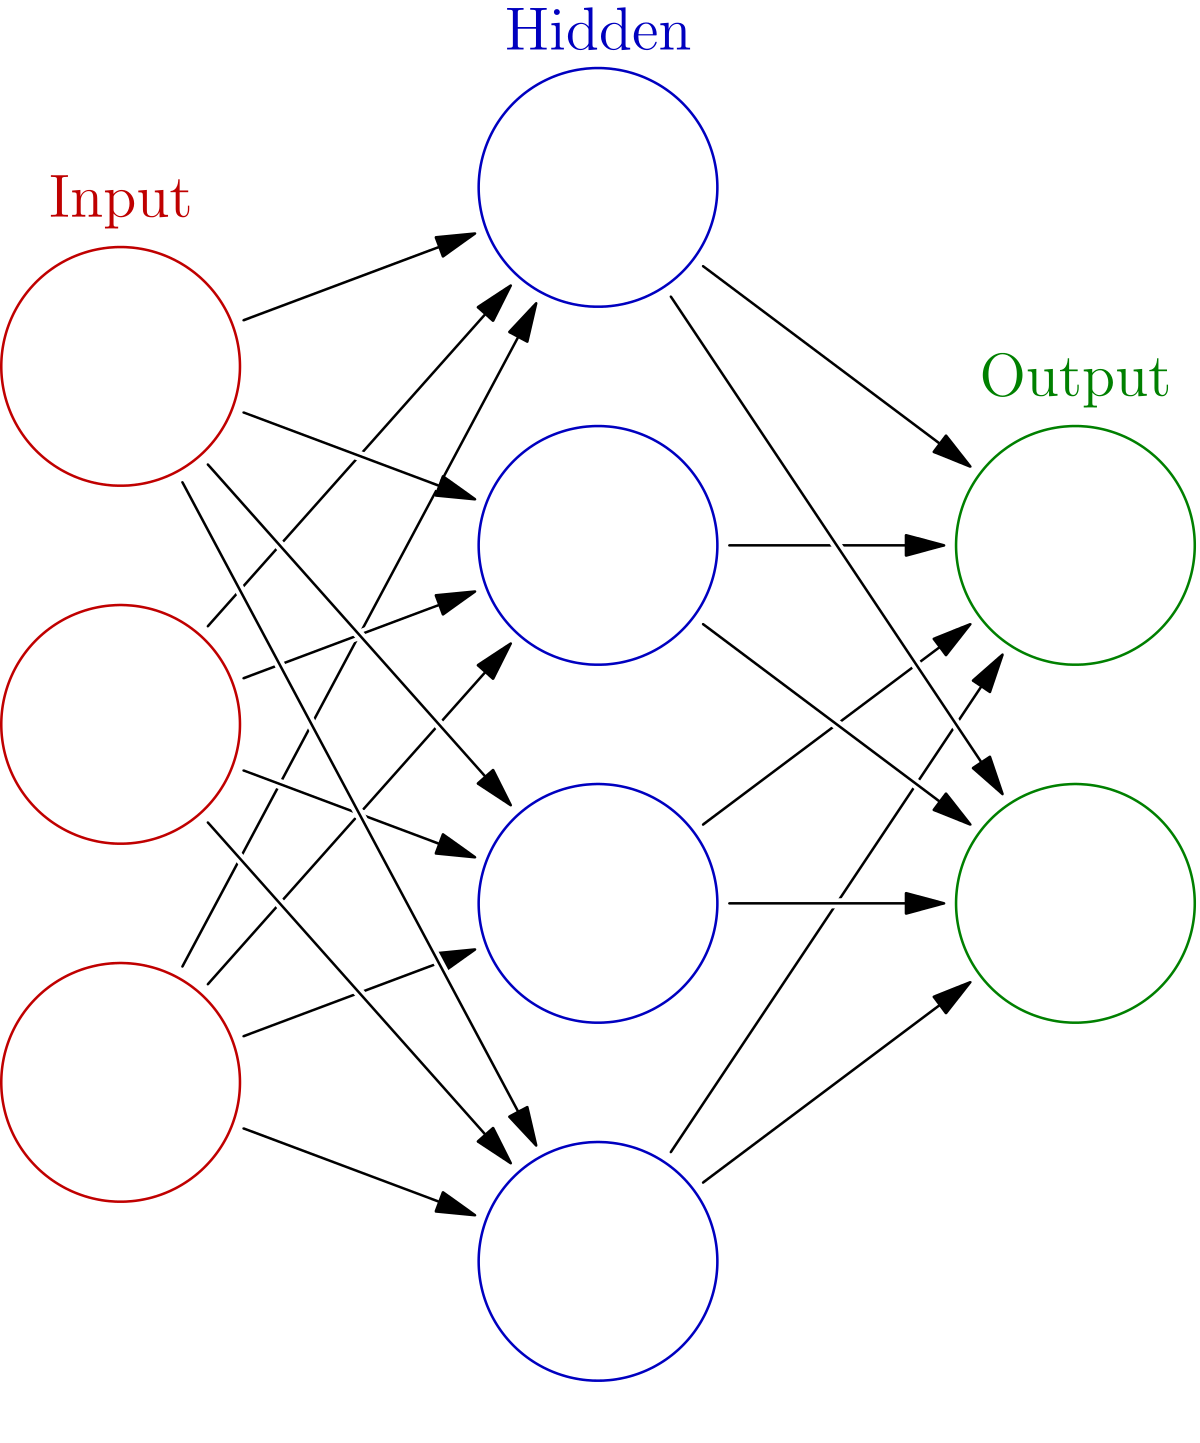
\includegraphics[width=8cm]{images/nn1.png}
  \caption{Neural network illustrated} % cite here
  \label{fig:nn1}
\end{figure}

\par The value of each neuron in the hidden and output layers is expressed by
\[k = \sigma(\sum_{i=1}^{n}(w_ia_i) + B)\]
where $k$ is the value of a neuron in the current layer, $w_i$ is the weight of the edge connecting the current neuron and the $i$th neuron from the previous layer, $a_i$ is the value of the $i$th neuron from the previous layer, and $B$ is a "bias" value.

\begin{figure}[H]
  \centering
  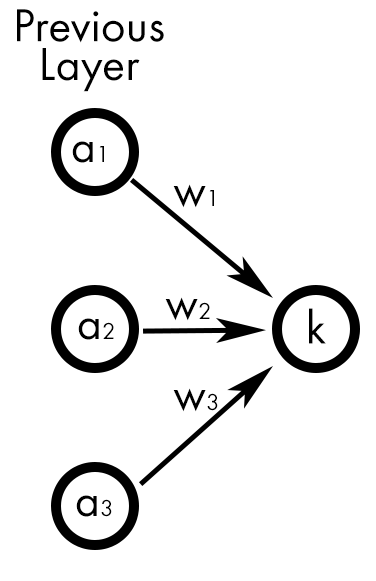
\includegraphics[width=5cm]{images/nn2.png}
  \caption{Illustration of the value of $k$} % cite here
  \label{fig:nn2}
\end{figure}

\par This phase can be done with linear algebra. If we look at the equation to find the value of a neuron in a layer, this is essentially multiplying a $m \times 1$ matrix to a $1 \times 1$ matrix. By extension, we can express the edges connecting one layer to another layer as a $m \times n$ matrix, with $m$ as the number of neurons in the current layer, and $n$ as the number of neurons in the previous layer. It will look something like so,
\begin{align*}
    \begin{bmatrix}
        w_{0,0} & w_{0,1} & \cdots & w_{0,n} \\
        w_{1,0} & w_{1,1} & \cdots & w_{1,n} \\
        \vdots & \vdots & \ddots & \vdots \\
        w_{m,0} & w_{m,1} & \cdots & w_{m,n}
    \end{bmatrix}
    \begin{bmatrix}
        a_0 \\
        a_1 \\
        \vdots \\
        a_n
    \end{bmatrix} &=
    \begin{bmatrix}
        k_0 \\
        k_1 \\
        \vdots \\
        k_m
    \end{bmatrix}.
\end{align*}
\par Thus, the equation for the value of some neuron $i$ is computed as follows:
\[k_i = \sigma(\sum_{j=1}^{n}(w_{i,j}a_{j}) + B_i).\]
% checking for error
\subsection{Checking for Error}
\par The values in the last layer would ideally contain the values on how the neural network classifies the input data. However, if the neural network is not that good, then it will wrongly classify the input data. Thus, it is important to check how much error the network made.
\par To do this, the input data must be accompanied with a correct answer so that the network would know how to respond when it sees the same thing again. There are multiple ways to check for the error of some output to some data, but for our implementation, we used the following equation:
\[\mathrm{error} = (k_i - c_i)^2 \]
where $c_i$ is the ideal value of the neuron.
\par If we manipulate the neural network in such a way so as to minimize the “wrongness” of each output, we can force it to "learn" from its mistakes, and this is where gradient descent is useful.

% propagate the error backwards (backward phase)
\subsection{Backward Phase}
\par Given that we know how much error the neural network produced with one forward phase, we have enough information to correct this mistake a bit. This will be done the same way how gradient descent is done. % WARNING: NOT DONE

% training the network
\subsection{Training the Network}
\par Now that we've learned about the forward and backward phase, we now know how a network learns. By feeding the neural network with input data with correct answers, we can "train" the network by letting it run the forward phase and it will be corrected by checking the error and it will attempt to fix the error with the backward phase.
\par With enough data training, the neural network should be modified enough to do what it has to do.

% arriving at an answer
\subsection{Getting an Answer}
\par With a trained network, looking at the values in the output layer will give us an answer. Each neuron would contain a value which represents how "similar" the input data is to its classification. Getting the maximum among the other neurons of the output layer would be the decision of the neural network.

% sample
\subsection{Sample Code in SageMath}
% WARNING: NOT DONE; insert the code and put some comments
\subsubsection{Neuron Class}
\lstinputlisting[caption={Neuron Class}]{neuronClass.py}
\subsubsection{Weight Class}
\lstinputlisting[caption={Weight Class}]{weightClass.py}
\subsubsection{Important Math Functions}
\lstinputlisting[caption={Important Math Functions}]{usefulMath.py}
\subsubsection{Gradient Multiply} % nate explain this in discussion
\lstinputlisting[caption={Gradient Multiply}]{gradientMul.py}
\subsubsection{Forward Phase}
\lstinputlisting[caption={Forward Phase}]{forwardPhase.py}
\subsubsection{Backward Phase}
\lstinputlisting[caption={Backward Phase}]{backPhase.py}
\subsubsection{Full Code}
\lstinputlisting[caption={Full Code}]{fullCode.py}

\section{Results}
% results of code?
\par To test the code if it's actually working, the following snippet of code was used. This may also be used as a template to provide further inputs.
\lstinputlisting[caption={Sample Input}]{exampleIn1.py}
\begin{figure}[H]
  \centering
  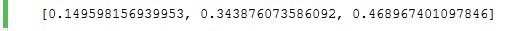
\includegraphics[width=12cm]{images/result1.png}
  \caption{Results of forward phase} % cite here
  \label{fig:result1}
\end{figure}

\section{Conclusion}
% WARNING: NOT DONE; summarize everything

\newpage
\printbibliography
\end{document}
